% !Mode::"TeX:UTF-8"
\documentclass[a4paper, 10pt]{article}
\usepackage{amssymb}
\usepackage{geometry}
\usepackage{graphicx}
\usepackage{fancyhdr}
\usepackage{setspace}
\usepackage{pdfpages}
\usepackage{listings}
\usepackage{amsthm}
\usepackage{authblk}
\usepackage{amsmath}
\usepackage{url}
\usepackage{hyperref}

\graphicspath{{./figure/}}

\geometry{left=2.5cm,right=2.5cm,top=2.5cm,bottom=2.5cm}

%\author{Chi Zhang\\\\Department of Computer Science\\\\University of Southern California}
\title{\textbf{Deep Reinforcement Learning for Portfolio Management}\thanks{Instructor: Joseph J. Lim}}
\author[]{Chi Zhang}
\author[]{Limian Zhang}
\author[]{Corey Chen}
\affil[]{Department of Computer Science}


\begin{document}

  \maketitle                     %generate the title
  \begin{spacing}{1.2}
    \section{Problem Definition}
    \subsection{Notations}
    In this project, we would like to manage portfolio by distributing our investment into a number of stocks based on the market. We define our environment similar to this paper \cite{DBLP:journals/corr/JiangXL17}.
    Concretely, we define $N$ to be the number of stocks we would like to invest.
    Without losing generality, at initial timestamp, we assume our total investment volume is 1 dollar. We define \emph{close/open relative price vector} as:
    \begin{equation}
    y_t=[1, \frac{v_{1,t, close}}{v_{1,t, open}}, \frac{v_{2,t, close}}{v_{2,t, open}},\cdots,\frac{v_{N,t,close}}{v_{N,t, open}}]
    \end{equation}
    where $\frac{v_{i, t, close}}{v_{i, t, open}}$ is the \emph{relative price} of stock $i$ at timestamp $t$. 
    Note $y[0]$ represents the relative price of cash, which is always 1. We define \emph{portfolio weight vector} as:
    \begin{equation}
    w_t=[w_{0,t}, w_{1, t}, \cdots, w_{N, t}]
    \end{equation}
    where $w_{i,t}$ represents the fraction of investment on stock $i$ at timestamp $t$ and $\sum_{i=0}^{N}w_{i, t}=1$. Note that $w_{0,t}$ represents the fraction of cash that we maintain. Then the profit after timestamp $T$ is:
    \begin{equation}
    \label{profit}
    p_T=\prod_{t=1}^{T}y_t\cdot w_{t-1}
    \end{equation}
    where $w_0=[1, 0, \cdots, 0]$. If we consider a trading cost factor $\mu$, then the trading cost of each timestamp is:
    \begin{equation}
    {\mu}_t=\mu\sum{|\frac{y_t \odot w_{t-1}}{y_t \cdot w_{t-1}} - w_{t}|}
    \end{equation}
    where $\odot$ is element-wise product. Then equation~\ref{profit} becomes:
    \begin{equation}
    \label{profit_mu}
    p_T=\prod_{t=1}^{T}(1-\mu_t) y_t\cdot w_{t-1}
    \end{equation}
    
    \subsection{Key Assumptions and Goal}
    To model real world market trades, we make several assumptions to simplify the problems:
    \begin{itemize}
      \item We can get any information about the stocks before timestamp $t$ for stock $i$. e.g. The previous stock price, the news and tweets online.
      \item Our investment will not change how the market behaves.
      \item The way we calculate profit in equation~\ref{profit} can be interpreted as: At timestamp $t$, we buy stocks according to the \emph{portfolio weight vector} $w_{t-1}$ computed by history data at \textbf{open} price and sell all the stocks at \textbf{close} price. This may not be true in practice because you will not always be able to \textbf{buy/sell} the stock at \textbf{open/close} price.
    \end{itemize}
    The \textbf{goal} of portfolio management is to maximum $p_T$ by choosing portfolio weight vector $w$ at each timestamp $t$ based on history stock information.
    
    \subsection{MDP formulation}
    \subsubsection{State and Action}
    We define state $s_t$ as $o_t$, where $o_t$ is the obseration of timestamp $t$. As the time goes by, the impact of history data decreases. Thus, we only consider the history price and news in a fixed window length $W$. Hence,
    \begin{equation}
    o_t=[\vec{v_{1,t}},\vec{v_{2,t}},\cdots,\vec{v_{N,t}}]
    \end{equation}
    where
    \begin{align}
    v_{i,t} &=\begin{bmatrix}
    v_{i,t-W} \\
    v_{i,t-W+1} \\
    \vdots \\
    v_{i,t-1}
    \end{bmatrix}
    \end{align}
    and $N$ is the number of stocks. The action $a_{t}$ is just \emph{portfolio weight vector} $w_{t}$. Note that this is a continuous state and action space problem. We try to directly solve it in continuous space instead of using discretization in previous work \cite{cs229_stanford_portfolio, cs229_stanford_trading}. Essentially, we want to train a policy network $\pi_\theta(a_t|o_t)$.
    \subsubsection{State Transition}
    The underlining state evolution is determined by the market, which we don't have any control. What we can get is the observation state, which is the price. Since we will collect history price of various stocks, $o_t$ is given by the dataset instead of $o_{t-1}$.\\
    \subsubsection{Reward}
    Instead of having reward 0 at each timestamp and $p_T$ at the end, we take logarithm of equation~\ref{profit_mu}:
    \begin{equation}
    \log{p_T}=\log{\prod_{t=1}^{T}\mu_t y_t\cdot w_{t-1}}=\sum_{t=1}^{T}\log(\mu_t y_t\cdot w_{t-1})
    \end{equation}
    Thus, we have $\log(\mu_t y_t\cdot w_{t-1})$ reward each timestamp, which avoids the sparsity of reward problem.
    
    \subsection{Datasets}
    \textbf{Stocks used:}
    We use 16 target stocks from NASDAQ100 that we feel are representative of different sectors in the index fund. They include "AAPL", "ATVI", "CMCSA", "COST", "CSX", "DISH", "EA", "EBAY", "FB", "GOOGL", "HAS", "ILMN", "INTC", "MAR", "REGN" and "SBUX".\\
    \textbf{Price Data:}
    We collected history price of the stocks from 2012-08-13 to 2017-08-11. The price on each day contains open, high, low and close. We use 2012-08-13 to 2015-08-12 as training data and 2015-08-13 to 2017-08-11 as testing data.\\
    \textbf{News Data:}
    We gather all tweets referencing the stocks from 2016-03-28 to 2016-06-15.\\
    \textbf{Additional Testing Data:}
    As another form of backtesting, we randomly select 16 stocks from NASDAQ100 the network has never seen and test whether the network generalizes.
    
    \section{Methods}
    We mainly consider model-free approach in our project. First, we train a predictor given a fixed history window length $W$ of price and news. With the predicted price, we can train a policy network $\pi_{\theta}(a_t|s_t)$ to maximize our portofolio value at the end of the trading period. Note that in practice, they are trained end-to-end instead of separately.
    
    \subsection{Data Preprocessing}
    \subsubsection{Numerical Data}
    Instead of using the raw open, high, low and close price, we normalize the history price as $(\frac{close}{open} - 1)\times scale$. There are two main advantages:
    \begin{enumerate}
      \item The history price are all in the same scale regardless of their actual price.
      \item Since the final portfolio is determined by the close/open ratio of each timestamp, it serves as a better feature compared with raw price.
    \end{enumerate}
    The \emph{scale} factor is heuristically set to 100 in our experiments. For missing data, we pad all open, high, low, close as the close price of previous day.
    \subsubsection{News Data}
    The steps to proprocess the news data are:
    \begin{enumerate}
      \item First, we filter each tweets by the most frequenct 2000 words.
      \item We pad each word with end of sentence mark to make them equally long.
      \item We use a sequence of end of sentence mark to fill the missing days.
    \end{enumerate}
    
    \subsection{Predictor Network}
    \begin{figure}
      \centering
      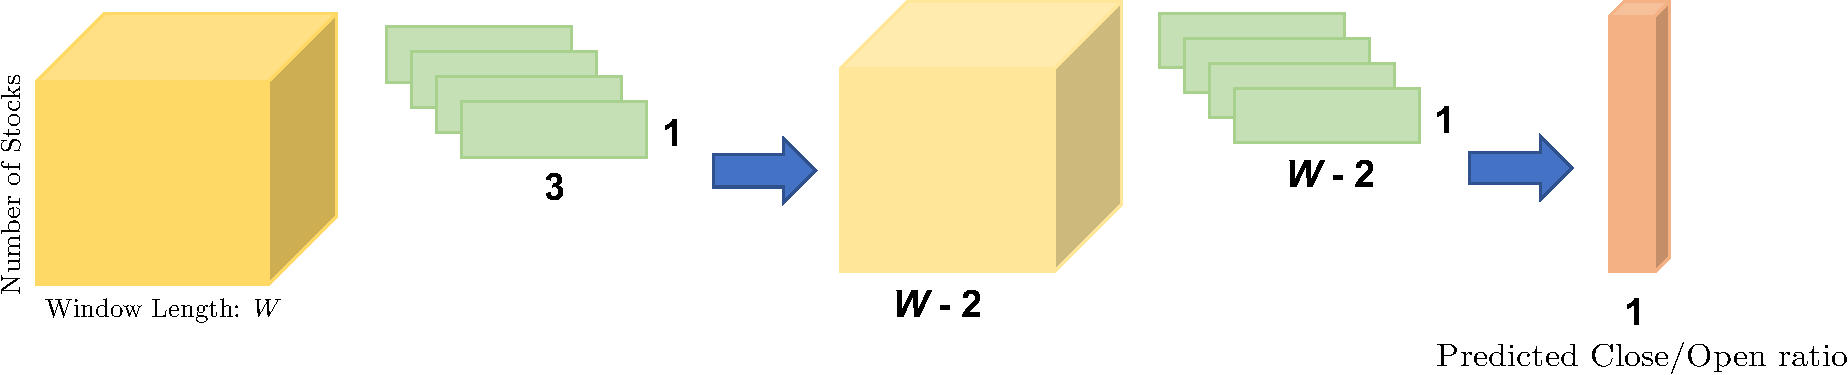
\includegraphics[scale=0.5]{predictor_cnn}
      \caption{CNN predictor based on numerical history}
      \label{fig:predictor_cnn}
    \end{figure}
  
    \begin{figure}
      \centering
      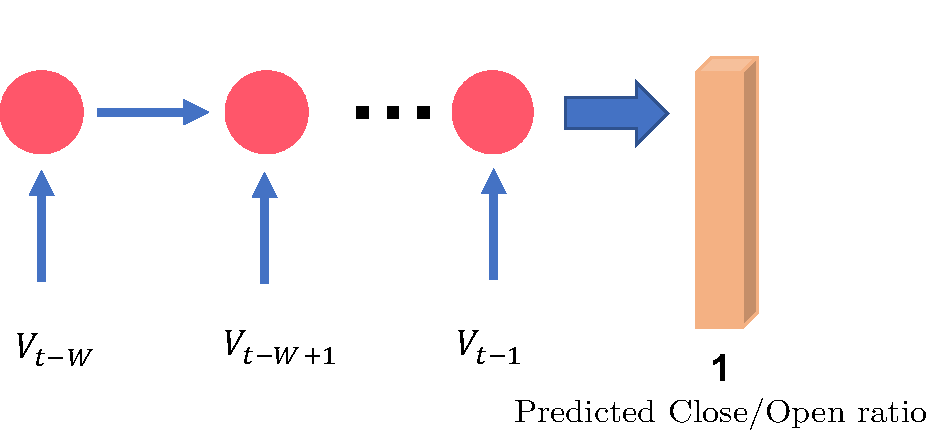
\includegraphics[scale=0.5]{predictor_lstm}
      \caption{LSTM predictor based on numerical history}
      \label{fig:predictor_lstm}
    \end{figure}
  
    \begin{figure}
      \centering
      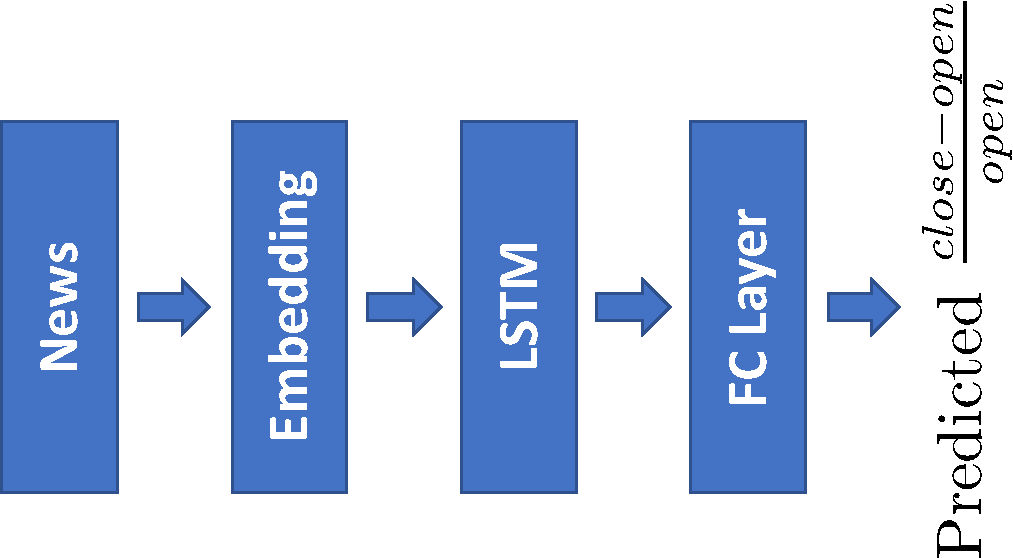
\includegraphics[scale=0.5]{predictor_lstm_news}
      \caption{LSTM predictor based on history of news}
      \label{fig:predictor_lstm_news}
    \end{figure}
    We show three predictors we train in Figure~\ref{fig:predictor_cnn}, Figure~\ref{fig:predictor_lstm} and Figure~\ref{fig:predictor_lstm_news}. The LSTM predictor based on numerical history is very straight forward. Note that all the stocks share the same LSTM. The rationale behind the CNN predictor is adpated from \cite{DBLP:journals/corr/JiangXL17}. For each timeseries of each stock, we use a $1\times3$ kernel to gather information in each window, then combine all the information to produce a single vector for each stock. Note that these convolutional windows doesn't cover information across any two stocks. For news based approach, we try to predict the $\frac{close-open}{open}$ ratio. We use pretrained 50d-GloVe to initialize the embedding layer followed by a LSTM and a fully-connected layer. 
    
    \subsection{Policy Network}
    \begin{figure}
      \centering
      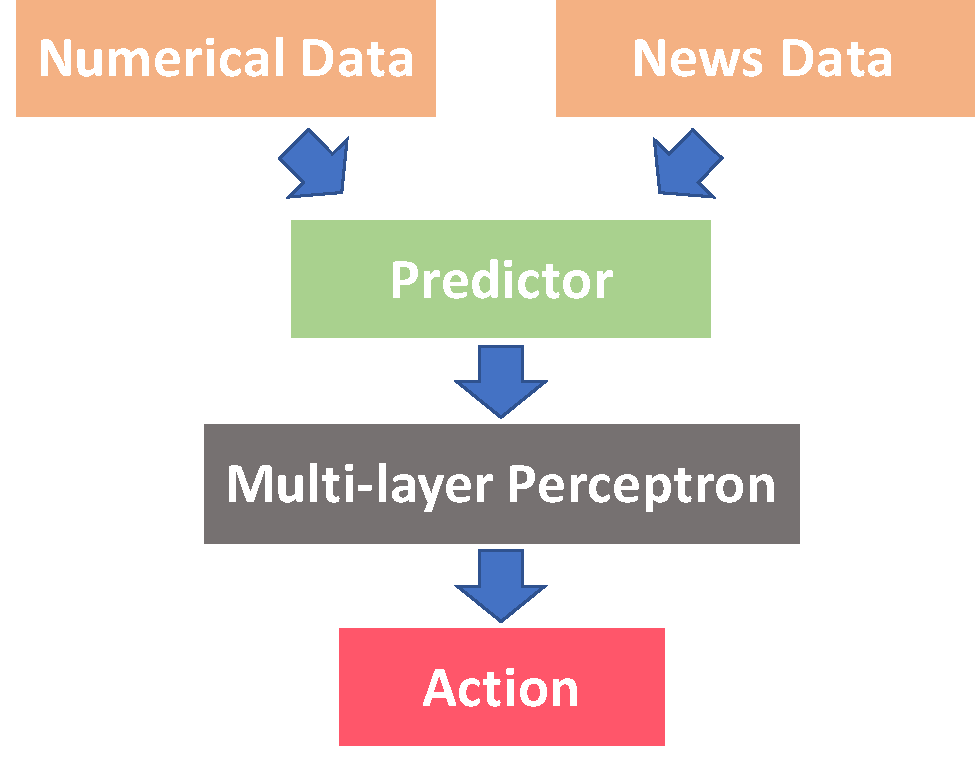
\includegraphics[scale=0.5]{actor}
      \caption{Policy Network}
      \label{fig:actor}
    \end{figure}
    We show the policy network topology in Figure~\ref{fig:actor}. All the policy network follows the same topology with different predictors.
    
    \subsection{Optimal Action and Imitation Learning}
    Suppose we know the stock price of tomorrow, we greedily choose the stock with the highest close/open ratio (taking into account trading cost of changing stocks), buying as much as possible on the open and selling all at the close.
    
    Given this fact, we can collect ground truth labels for each timestamp by choosing the optimal action. (e.g. $[0, 0, 1, \cdots, 0, 0]$, the stock with highest close/open to be 1 and all the others to be 0) Then, we can train a policy network by imitating optimal action conditioned on the current state $s_t$. The policy network is a three layer MLP.
    
    \subsection{Deep Deterministic Policy Gradient (DDPG)}
    We try to directly learn a policy network $\pi_{\theta}(a_t|s_t)$ by continuous action space reinforcement learning algorithm~\cite{DBLP:journals/corr/LillicrapHPHETS15}. We show the algorithm in Figure~\ref{fig:ddpg_algorithm}. The configurations are:
    \begin{figure}
      \centering
      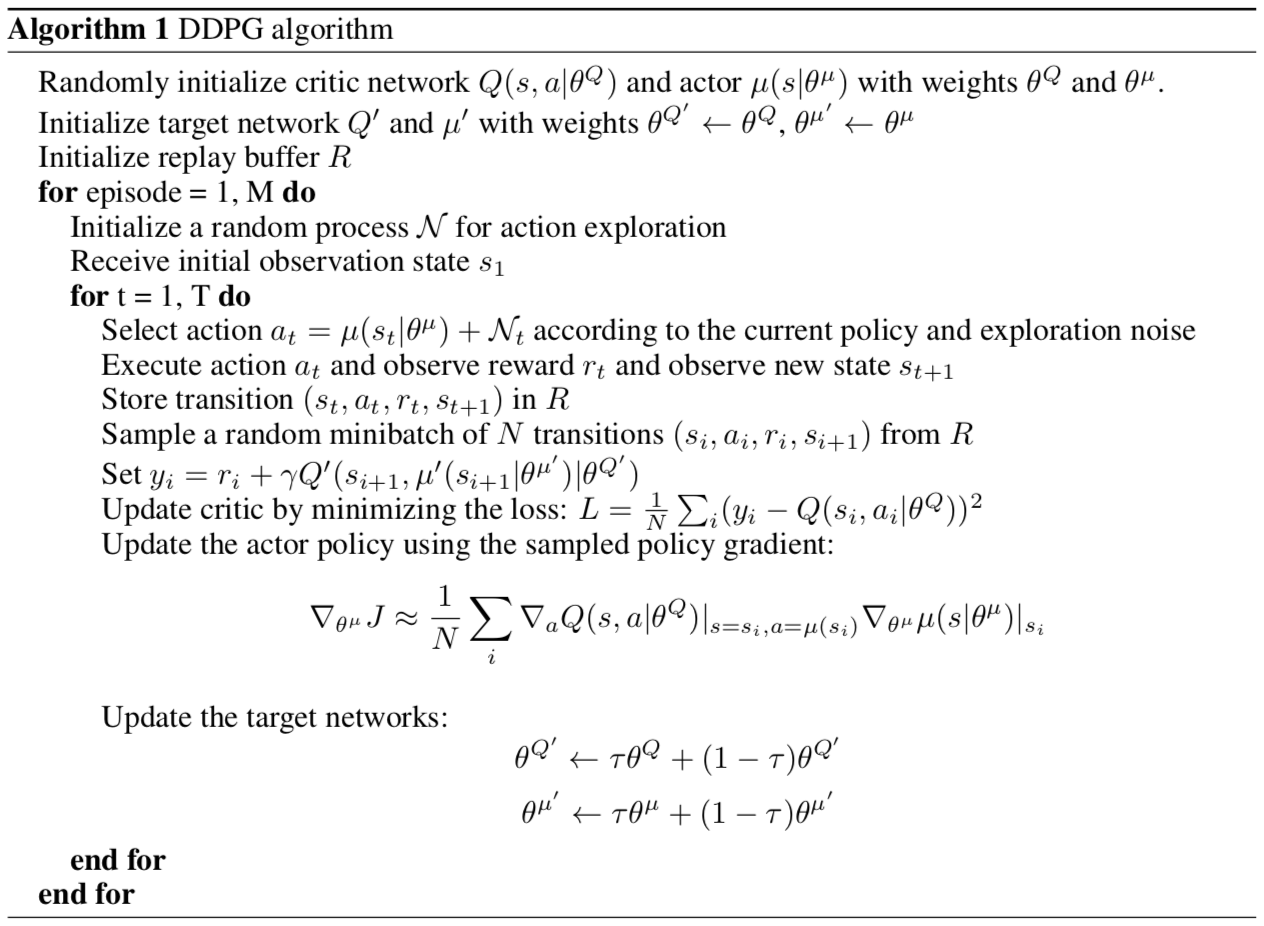
\includegraphics[scale=0.5]{ddpg}
      \caption{Deep Deterministic Policy Gradient Algorithm\cite{DBLP:journals/corr/LillicrapHPHETS15}}
      \label{fig:ddpg_algorithm}
    \end{figure}
    \begin{itemize}
      \item Actor Network: predictor in Section 2.2 plus a three layer perceptron.
      \item Critic Network: a linear combination of actor network structure of state (observation) and action.
      \item Exploration noise: Ornstein-Uhlenbeck with zero mean, 0.3 sigma and 0.15 theta.
      \item For fairness, we train models with different settings in 500 episodes. Some of the models are not fully converged at that time though. 
    \end{itemize}
    
    \section{Results}
    \subsection{Imitation learning}
    \begin{figure}[htbp]
      \centering
      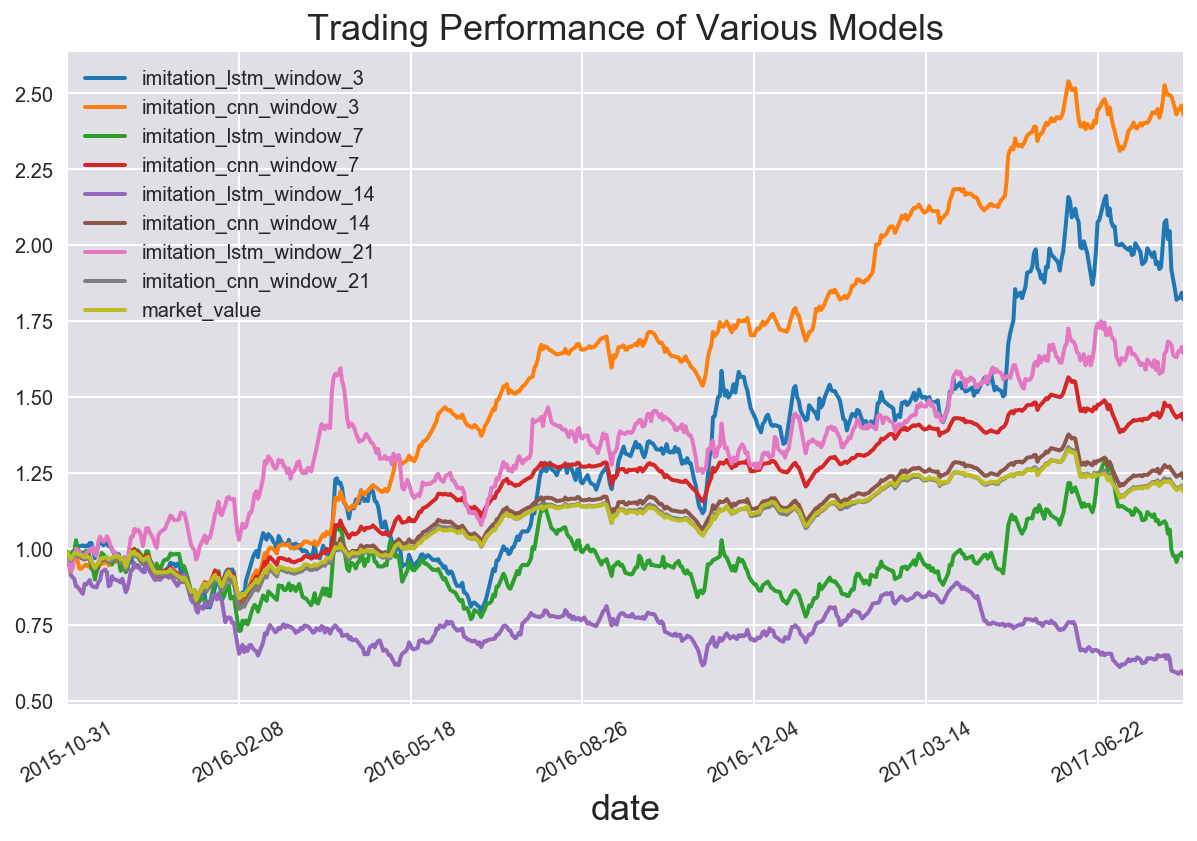
\includegraphics[scale=0.7]{imitation_result}
      \caption{Results of trading on testing data using policy trained by imitation learning}
      \label{fig:imitation_learning}
    \end{figure}
    We show the result of trading on testing data using policy trained by imitation learning in Figure~\ref{fig:imitation_learning}. The market value is obtained by equally distributing your investment to all the stocks. It turns out that smaller windows work better. Larger window means larger models and it tends to overfit very quickly since the training data is just around 1000.
    
    \subsection{DDPG}
    \begin{figure}[htbp]
      \centering
      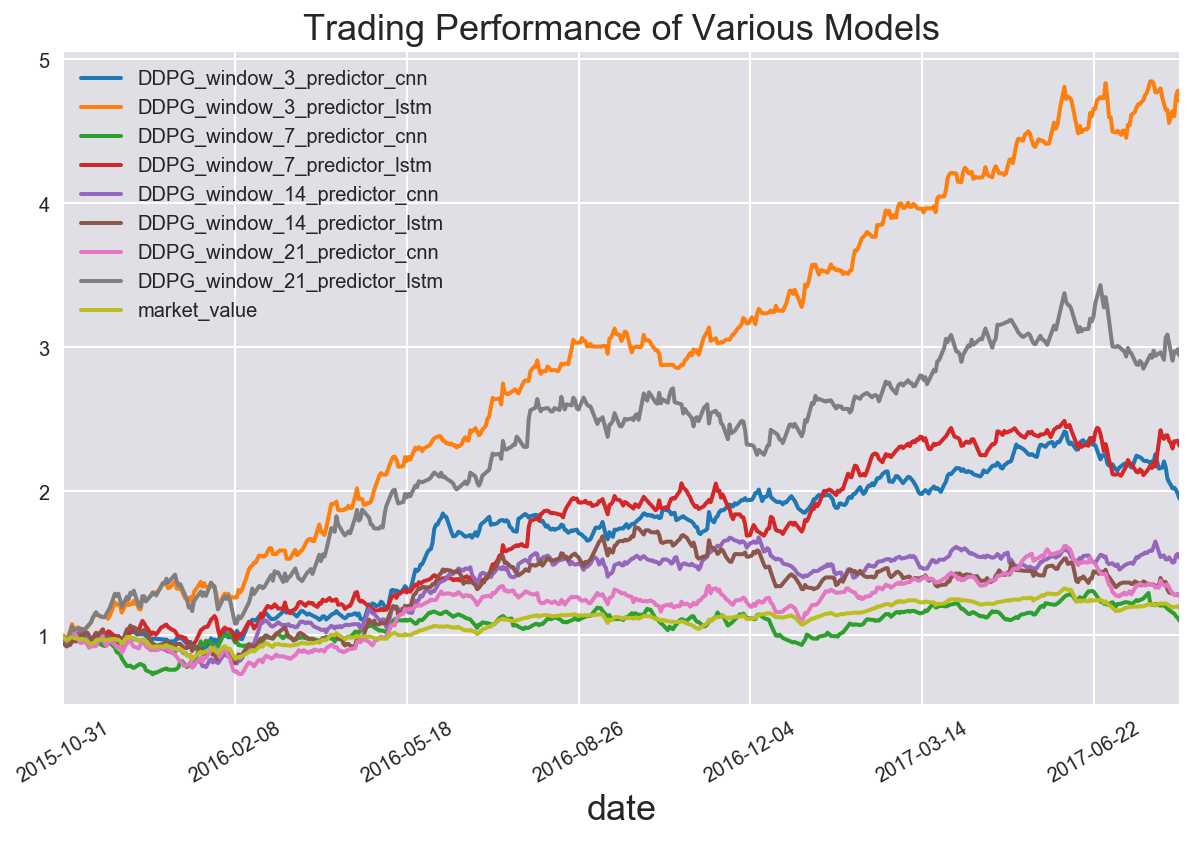
\includegraphics[scale=0.7]{ddpg_result}
      \caption{Results of trading on testing data using policy trained by DDPG}
      \label{fig:ddpg}
    \end{figure}
    We show the result of trading on testing data using policy trained by DDPG in Figure~\ref{fig:ddpg}. We find that LSTM predictor based models have better performance than the CNN predictor based models. It is not surprising that smaller windows perform best because of the temporaral relationship among price in a short window.
    
    \subsection{Imitation vs DDPG}
    \begin{figure}
      \centering
      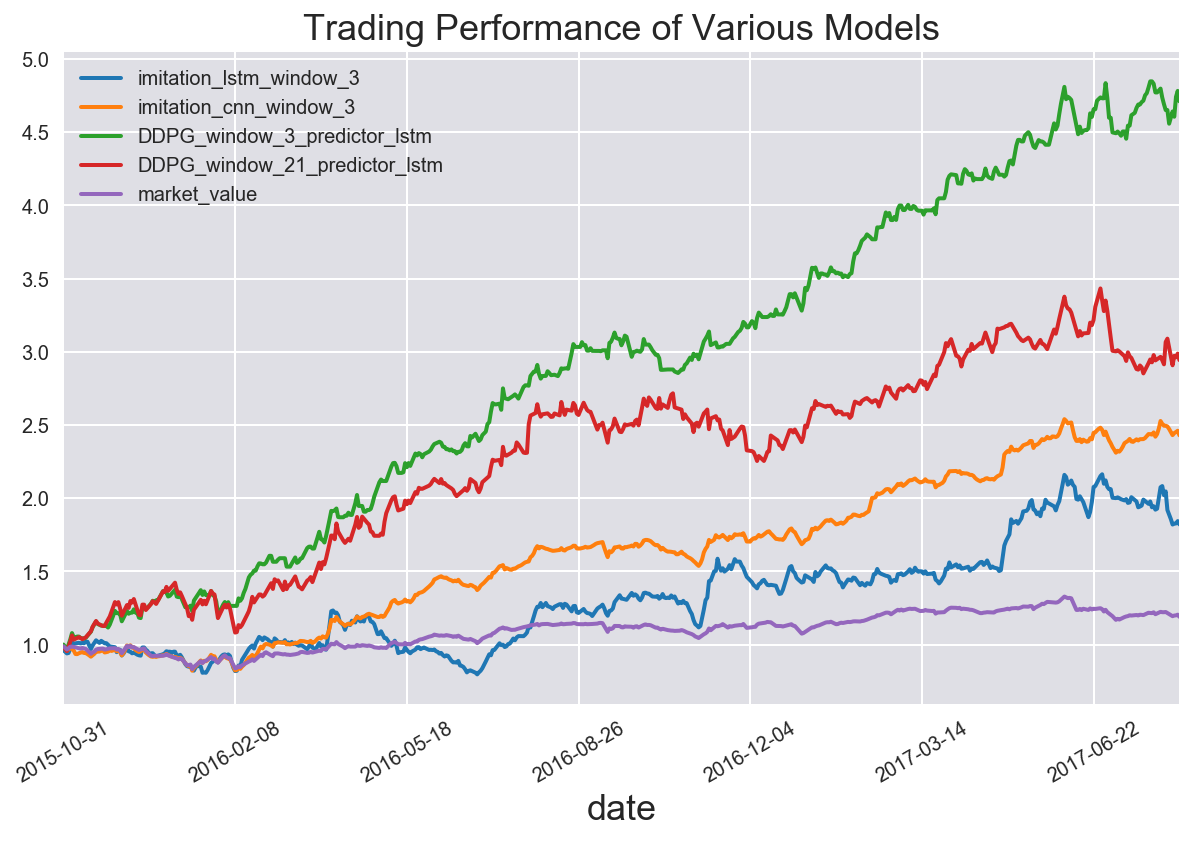
\includegraphics[scale=0.7]{imitation_vs_ddpg}
      \caption{Results of trading on testing data using best two networks trained by imitation learning and DDPG}
      \label{fig:imitation_vs_ddpg}
    \end{figure}
    Generally, models trained by DDPG is better than models trained by imitation learning as shown in figure~\ref{fig:imitation_vs_ddpg}. The problem of training good networks by imitation learning is the extreme prone to overfitting while DDPG doesn't suffer from this problem because each episode is sampled from the whole training period with different starting date and lengths.
%    
%    \subsection{Numerical input vs news input}
%    
%    \subsection{Unseen stocks}
    
    \subsection{Related Work}
    In \cite{cs229_stanford_portfolio, cs229_stanford_trading}, the author proposes to use DQN to trade in 2 stocks market with discreted state and action space. Their settings are far simpler than ours. In \cite{DBLP:journals/corr/JiangXL17}, the author proposes to use Deterministic Policy Gradient (DPG) to trade in bitcoin market. It's very hard to compare with them because of different dataset. But DDPG is strictly better than DPG in terms of performance and convergence time.
    
    \section{Contribution}
    \textbf{Chi Zhang:} 
    \begin{itemize}
      \item Collect and preprocess stock price.
      \item Set up environment (OpenAI gym).
      \item Train DDPG model.
      \item Write report.
    \end{itemize}
    \textbf{Corey Chen:}
    \begin{itemize}
      \item Compute optimal action
      \item Train CNN and LSTM policy network using imitation learning.
    \end{itemize}
    \textbf{Limian Zhang:}
    \begin{itemize}
      \item Collect and preprocess tweets datasets.
      \item Predict future stock price based on history price and tweets data.
    \end{itemize}
    
    
%    
%    \begin{figure}
%      \centering
%      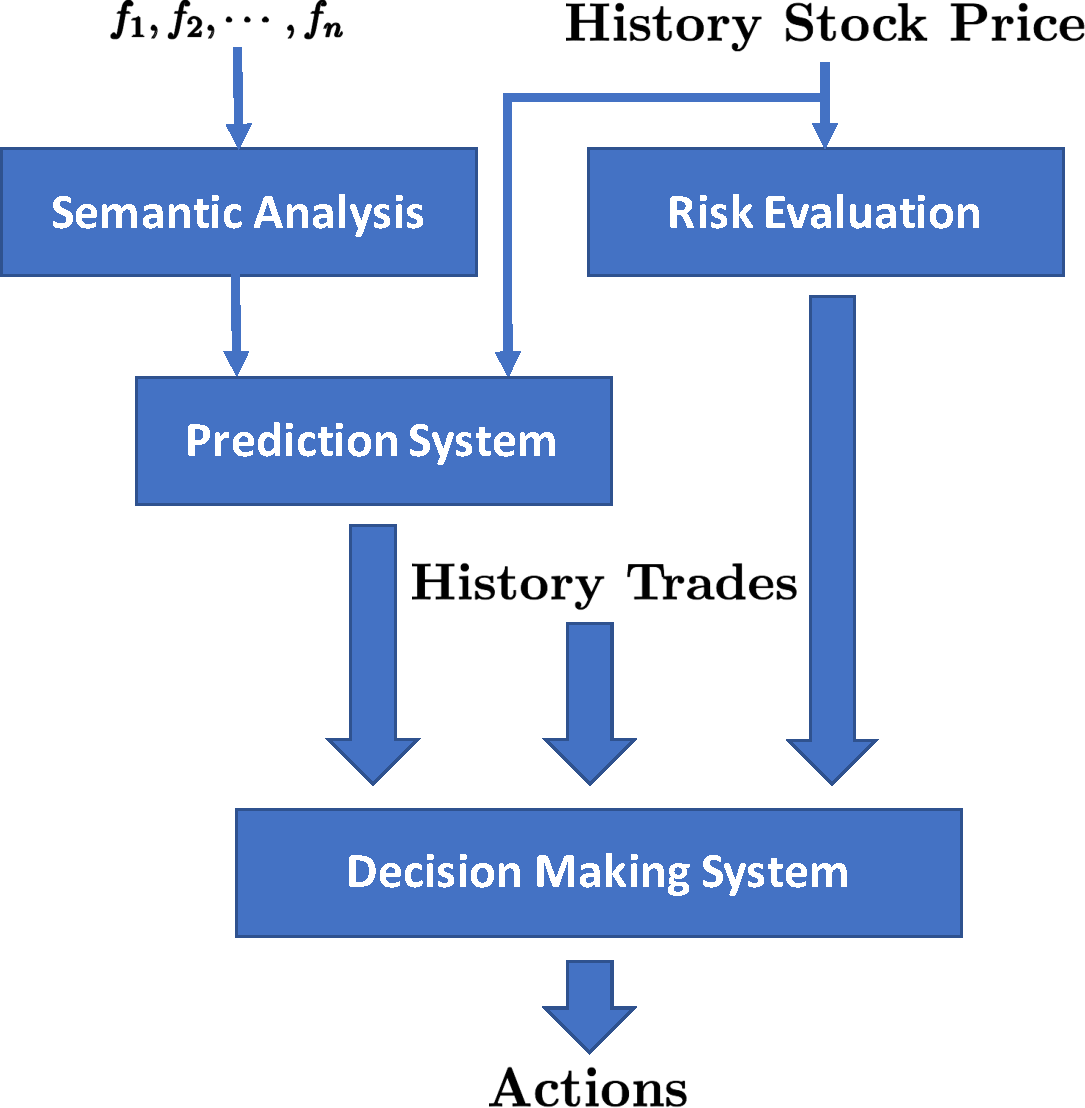
\includegraphics[width=0.4\textwidth]{diagram}
%      \caption{Digram of proposed approach}
%      \label{diagram_approach}
%    \end{figure}
    
    
  
  \end{spacing}  

  \bibliographystyle{IEEEtran}
  \bibliography{./bib/stock_prediction.bib}

\end{document}
